\let\negmedspace\undefined
\let\negthickspace\undefined
\documentclass[journal]{IEEEtran}
\usepackage[a5paper, margin=10mm, onecolumn]{geometry}
%\usepackage{lmodern} % Ensure lmodern is loaded for pdflatex
\usepackage{tfrupee} % Include tfrupee package

\setlength{\headheight}{1cm} % Set the height of the header box
\setlength{\headsep}{0mm} % Set the distance between the header box and the top of the text

\usepackage{gvv-book}
\usepackage{gvv}
\usepackage{cite}
\usepackage{amsmath,amssymb,amsfonts,amsthm}
\usepackage{algorithmic}
\usepackage{graphicx}
\usepackage{textcomp}
\usepackage{xcolor}
\usepackage{txfonts}
\usepackage{listings}
\usepackage{enumitem}
\usepackage{mathtools}
\usepackage{gensymb}
\usepackage{comment}
\usepackage[breaklinks=true]{hyperref}
\usepackage{tkz-euclide} 
\usepackage{listings}
% \usepackage{gvv}                                        
\def\inputGnumericTable{}                                 
\usepackage[latin1]{inputenc}                                
\usepackage{color}                                            
\usepackage{array}                                            
\usepackage{longtable}                                       
\usepackage{calc}                                             
\usepackage{multirow}                                         
\usepackage{hhline}                                           
\usepackage{ifthen}                                           
\usepackage{lscape}
\begin{document}

\bibliographystyle{IEEEtran}
\vspace{3cm}

\title{2.4.29}
\author{EE25BTECH11033 - Kavin}
% \maketitle
% \newpage
% \bigskip
{\let\newpage\relax\maketitle}

\renewcommand{\thefigure}{\theenumi}
\renewcommand{\thetable}{\theenumi}
\setlength{\intextsep}{10pt} % Space between text and floats
\textbf{Question}:\\
The points $\vec{A}(2, 9), \vec{B}(a, 5) $ and $\vec{C}(5, 5)$ are the vertices of a triangle $\vec{ABC}$ right angled at $\vec{B}$. Find the values of a and hence the area of $\triangle \vec{ABC}$.\\
\bigskip

\textbf{Solution}:\\
Given the points,
\begin{align}
    \vec{A}=\begin{myvec}{2\\9}\end{myvec}\ \ 
    \vec{B}=\begin{myvec}{a\\5}\end{myvec}\ \ 
    \vec{C}=\begin{myvec}{5\\5}\end{myvec}
\end{align}
Also it is given that the triangle $\vec{ABC}$ right angled at $\vec{B}$.\\
\\
$\therefore$ The vectors $(\vec{A}-\vec{B})$ and $(\vec{C}-\vec{B})$ are perpendicular.\\
\\
The angle $\theta$ between vectors $(\vec{A}-\vec{B}), (\vec{C}-\vec{B})$, is given by 
\begin{align}
	\label{eq:angle-inner}
		\cos\theta=\frac{{(\vec{A}-\vec{B})^{\top}}{(\vec{C}-\vec{B})}}{\norm{\vec{A}-\vec{B}}\norm{\vec{C}-\vec{B}}}
\end{align}
\bigskip
\\
Here $\theta$ = $90\degree$.

\begin{align}
\implies {(\vec{A}-\vec{B})^{\top}}{(\vec{C}-\vec{B})} = 0
\end{align}\\
\begin{center}
$\vec{A}$ - $\vec{B}$ = $\myvec{2-a\\4}$
\end{center}
\begin{center}
$\vec{C}$ - $\vec{B}$ = $\myvec{5-a\\0}$
\end{center}\\
\begin{align}
    \myvec{2-a\\4}^{\top}\myvec{5-a\\0} = 0\\
    \myvec{2-a & 4}\myvec{5-a\\0} = 0\\
    \implies \brak{2-a}\brak{5-a} + \brak{4\times0} = 0\\
    \implies \brak{2-a}\brak{5-a} = 0
\end{align}
\begin{align}
    \implies a = 2
\end{align}
\\
Here $a = 5$ is not considered because when $a = 5$, the points $\vec{B}$ and $\vec{C}$ will be the same and hence a triangle cannot be formed.\\
\begin{center}
$\vec{B}=\begin{myvec}{2\\5}\end{myvec}$
\end{center}
The area of $\triangle ABC$ is given by
		\begin{align}
			Area = \frac{1}{2}\norm{{\brak{\vec{A}-\vec{B}}\times \brak{\vec{A}-\vec{C}}}}
		\end{align}
\begin{center}
    \brak{\vec{A}-\vec{B}} =$\myvec{0\\4}$\\
    \brak{\vec{A}-\vec{C}} = $\myvec{-3\\4}$
\end{center}
\\
\begin{align}
\implies Area = \frac{1}{2}\norm{\myvec{0\\4}\times \myvec{-3\\4}}
\end{align}
\begin{align}
\implies Area = \frac{1}{2}\norm{0 + 12}
\end{align}
\begin{align}
\implies Area = 6
\end{align}\\
Hence the area of $\triangle \vec{ABC}$ is $6$ sq.units.\\
See Fig. 0 ,
\begin{figure}[H]
\begin{center}
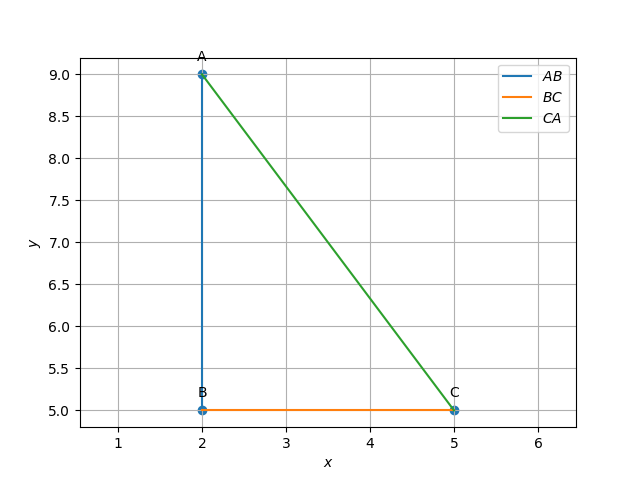
\includegraphics[width=0.6\columnwidth]{figs/fig.png}
\end{center}
\caption{}
\label{fig:Fig1}
\end{figure}
\end{document}